\section{Ergebnisse der Betriebsszenarien}
In dem Kapitel \ref{s:Betriebsszenarien} wurden drei Szenarien für den Vergleich aufgestellt, in diesem Abschnitt werden sie ausgewertet und
miteinander verglichen. Wobei erstens werden die Betriebskosten unter sich verglichen, zweitens die benötigten Infrastrukturkosten für jedes Szenario
und schließlich werden die Szenarien mit der Berücksichtigung beider Aspekte angeschaut.

\textit{Betriebskosten}
Die Flottenaufteilung nach Szenarien kann in der folgenden Tabelle zusammengefasst werden:
\begin{table}[h]
	\begin{center}
    \caption{Werte und Annahmen der BA-Infrastruktur}
	\label{BA_Infrastrukturtab}
	\begin{tabular}{|c|c|c|>{\centering\arraybackslash}p{3cm}|c|}
		\hline
		\multicolumn{4}{|c|}{\textbf{Szenario I}} \\ \hline
		 & \textbf{Batterieantrieb} & \textbf{Wasserstoffantrieb} & \textbf{SAF} \\ \hline
		Kurzstrecken & 422 & - &-\\ \hline
      	Mittelstrecken & -  & 54 &- \\ \hline
		Langstrecken & - & - &104 \\ \hline
		\multicolumn{4}{|c|}{\textbf{Szenario II}} \\ \hline
		Kurzstrecken & 211 &- &211\\ \hline
      	Mittelstrecken &  - & 54 &- \\ \hline
		Langstrecken &- & 46  &58 \\ \hline
		\multicolumn{4}{|c|}{\textbf{Szenario III}} \\ \hline
		Kurzstrecken & 290 &- &132\\ \hline
      	Mittelstrecken &  - & 27 & 27 \\ \hline
		Langstrecken &  -& 52 &52 \\ \hline
	\end{tabular}
    \end{center}
\end{table}

Obwohl der Unterschied zwischen Betriebskosten gleichmäßig ist, hat unter allen Betriebsszenarien das zweite die höchsten Gesamtbetriebskosten (siehe Abb. \ref{res_betriebsszenarien}). 
Erstes gegenüber hat die geringsten Kosten. Werden, das zweite Szenario ist 3,5 \% teuer als das erste.
Zweites Szenario: Großteil (58 \%) der Kosten entsteht durch wasserstoffbetriebene-Flugzeuge. Weitere 36 \% verursacht den SAF.
Erstes Szenario hat der niedrigste Betriebswert von allen drei. Die Kosten des ersten Szenarios teilen sich folgend aus. 
Betrieb mit der SAF verursacht in diesem Szenario die meisten Kosten. Etwa ein Drittel
der Kosten sind von dem Betrieb mit Wasserstoff verbunden.
Das dritte Szenario hat 1 \% geringere Kosten als das zweite.
Erkennbar ist auch, dass die Betriebskosten, die durch am Batterieantrieb verursacht am geringsten unter allen Szenarien sind.
\begin{figure}[h]
	\centering
	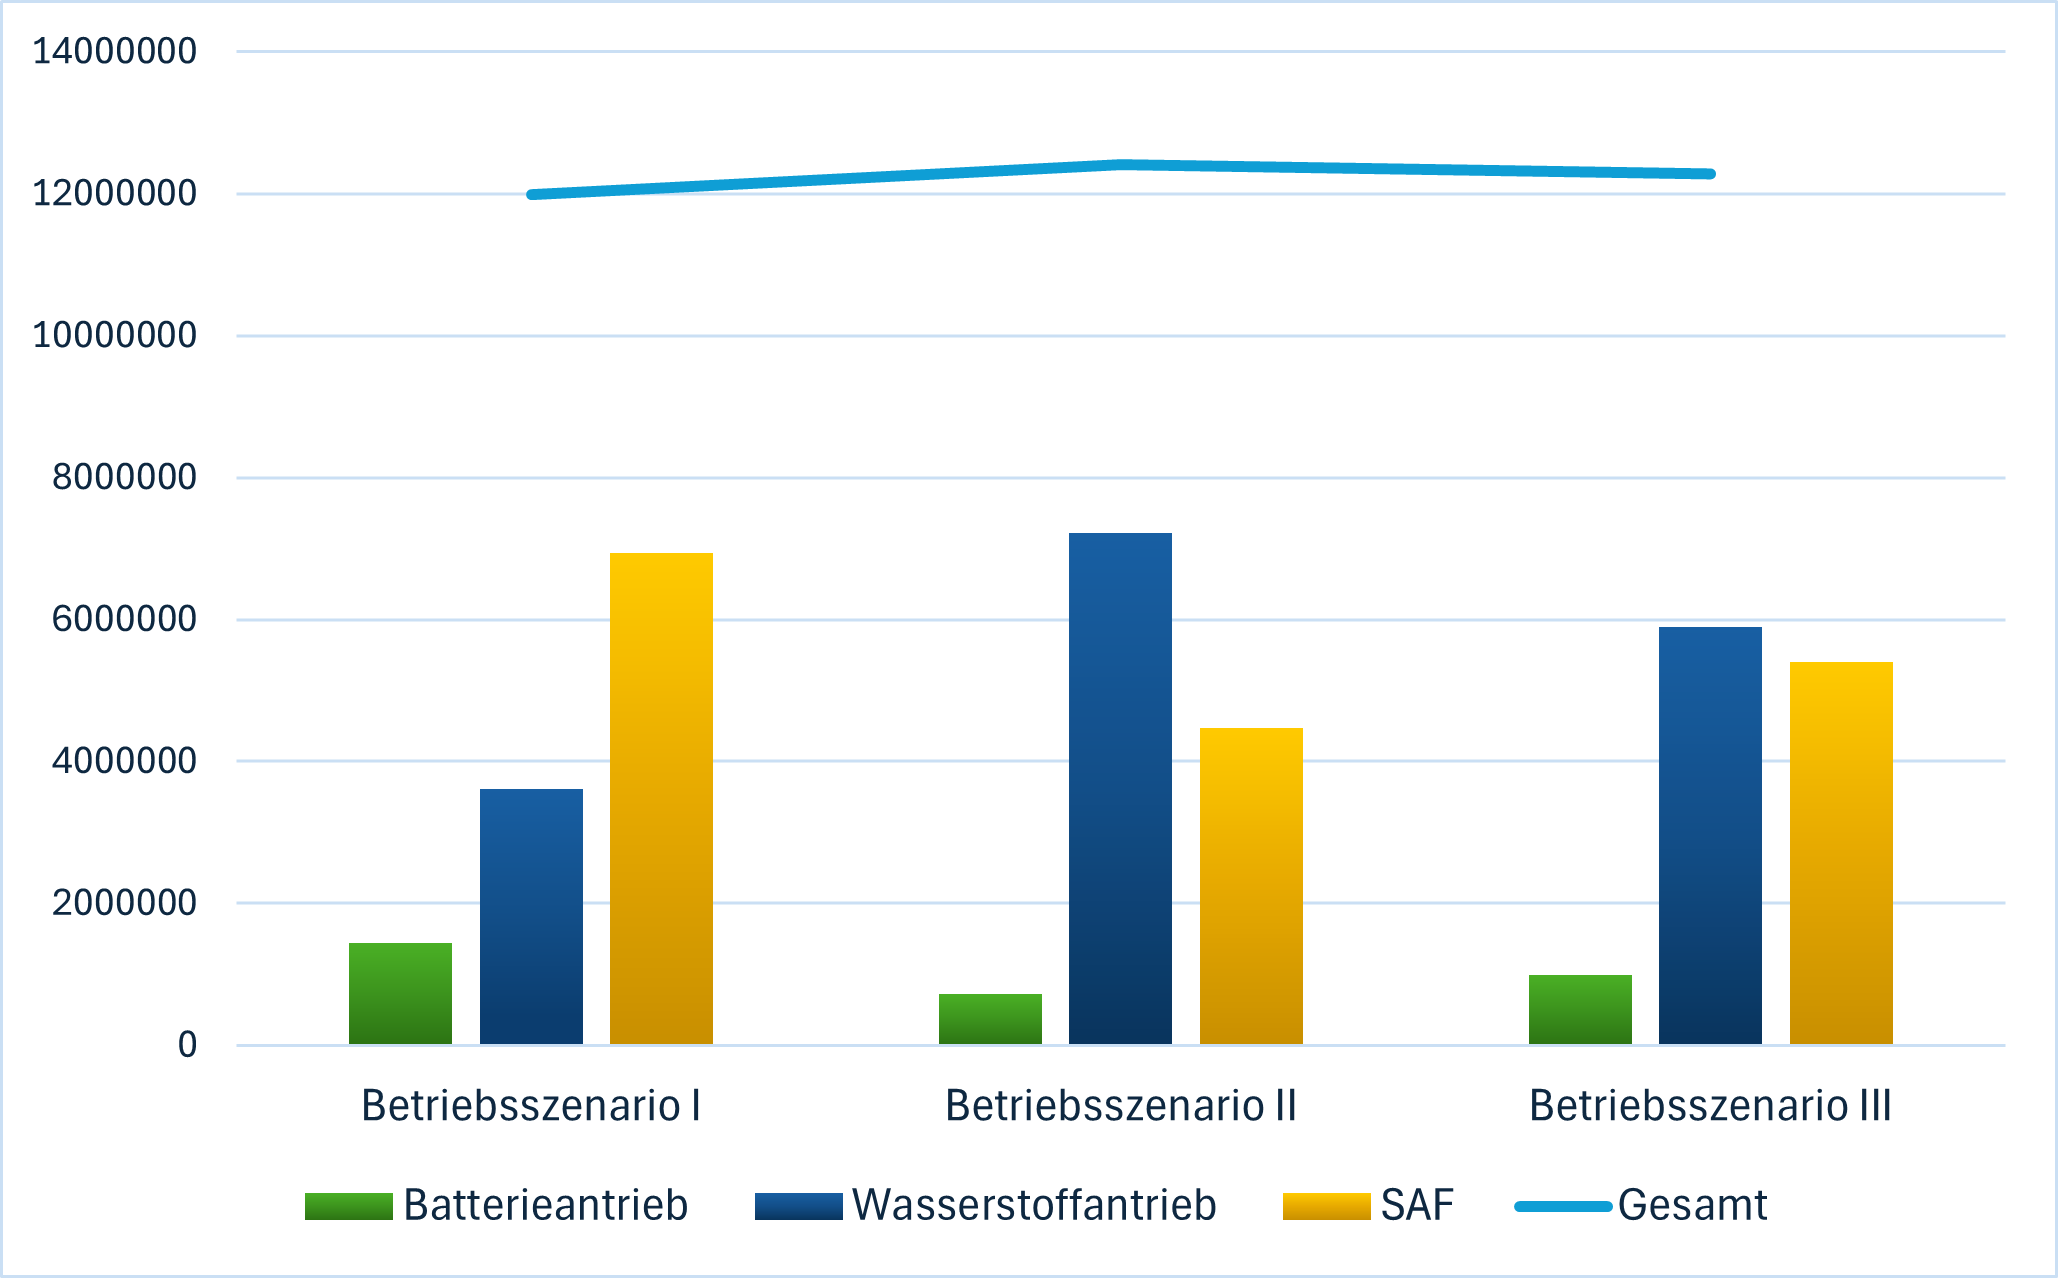
\includegraphics[width=0.8\linewidth]{Bilder/betriebssz_res.png}
	\caption[Betriebskosten in Abhängigkeit von Szenarien mit Gesamtkostentrend]{Betriebskosten in Abhängigkeit von Szenarien mit Gesamtkostentrend}
	\label{res_betriebsszenarien}
\end{figure}

\textit{Infrastrukturkosten}\\
Nennenswert ist, dass in der Berechnung von allen Betriebsszenarien erstmal nur einmalige Infrastrukturausgaben 
ohne jährliche Abschreibungen ausgerechnet sind. In der Tabelle \ref{Infrastrukturwerte_res} sind die benötigten 
Infrastrukturanschaffungswerte für jedes Szenario zusammengefasst. 

\begin{table}[h]
	\begin{center}
    \caption{Infrastrukturwerte für Wasser- und Batterieantrieb für alle Szenarien}
	\label{Infrastrukturwerte_res}
	\begin{tabular}{|l|c|c|c|}
		\hline
		 & \textbf{Szenario I}& \textbf{Szenario II}& \textbf{Szenario III} \\ \hline
		Anzahl Ladestationen $n_{BSS}$ & 20 & 10& 14\\ \hline
		Anzahl Batterien $n_{Bat}$ & 101 & 51& 70 \\ \hline
		Anzahl Betankungswagen $n_{BW}$ & 4 & 7 & 5\\ \hline
		Anzahl Pumpen $n_{kP}$  & 5 & 8 & 6\\ \hline
	\end{tabular}
    \end{center}
\end{table}

Das erste Szenario hat die kleinsten Ausgaben, wobei das zweite Szenario die größte und 27 \% höher als das erste.
Die Gesamtkosten für das zweite Szenario liegen über 35 Tausend Euro.
\begin{figure}[h]
	\centering
	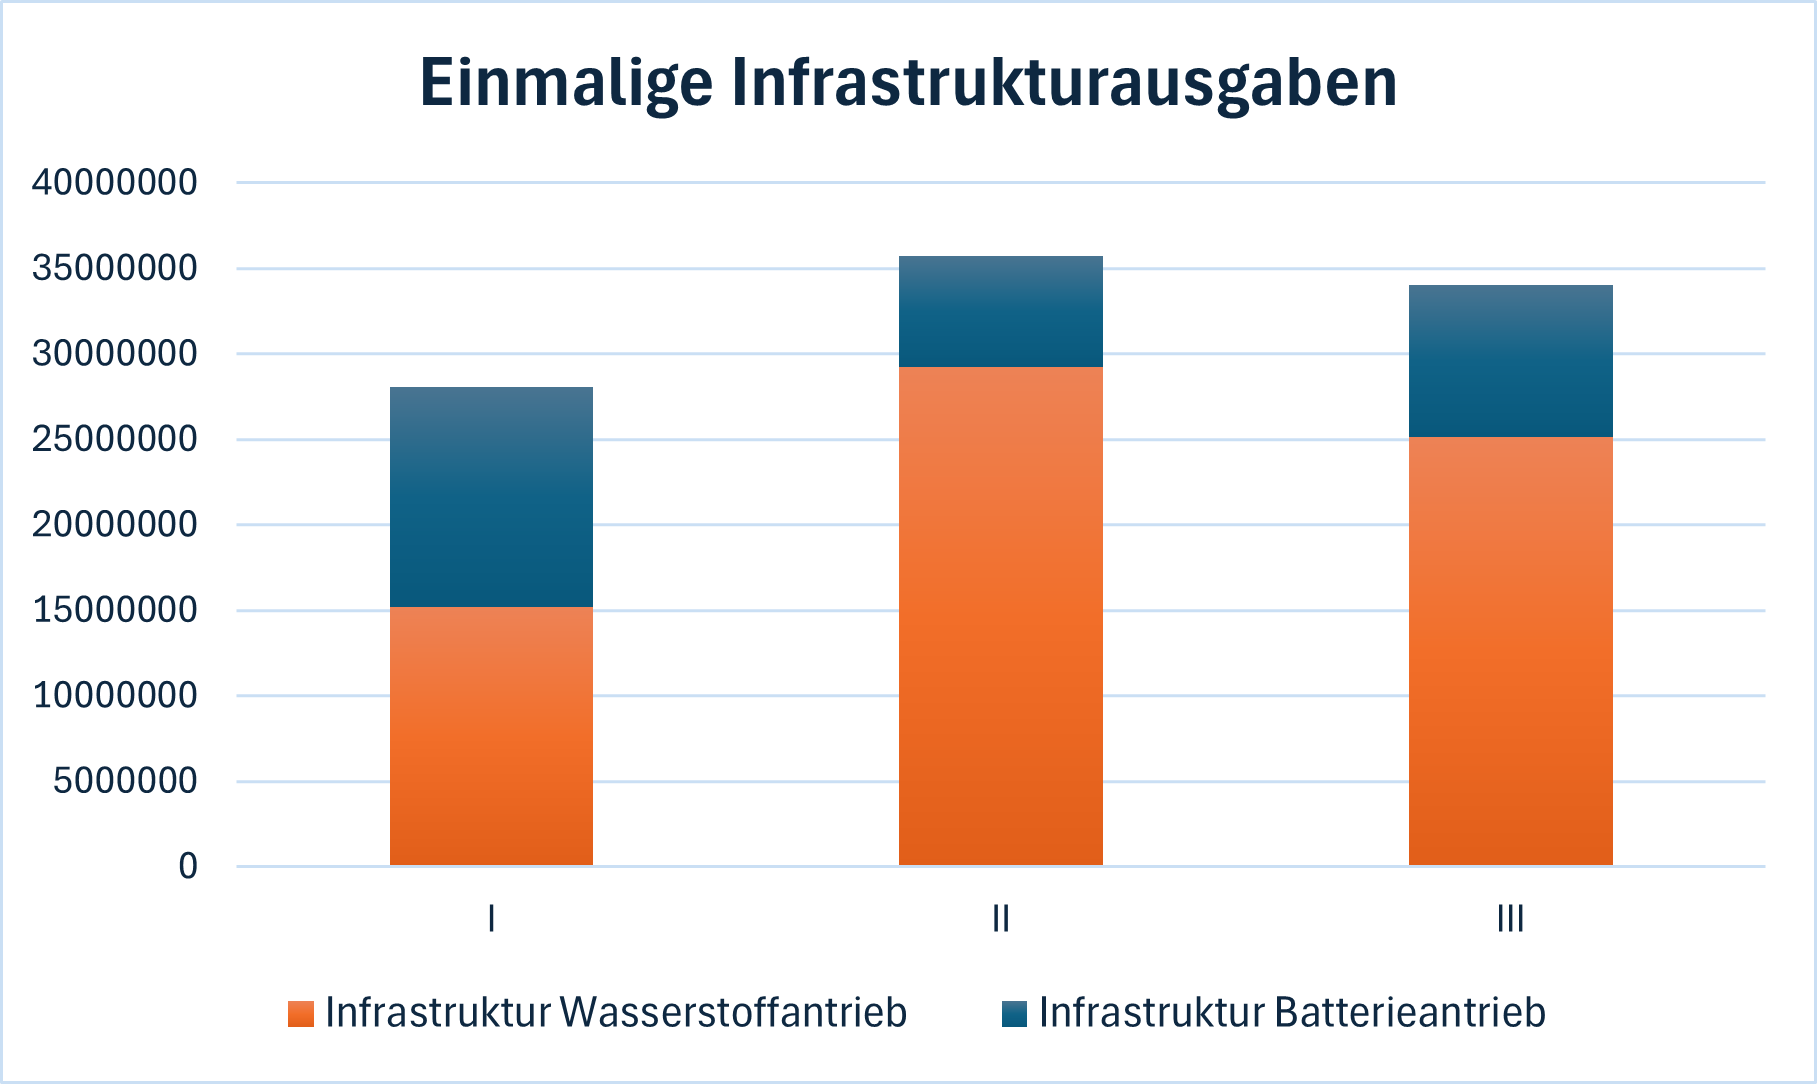
\includegraphics[width=0.8\linewidth]{Bilder/Infr_Szenarien.png}
	\caption[Betriebsszenarien]{Vergleich der einmaligen Infrastrukturausgaben zwischen den Betriebsszenarien}
	\label{res_betriebsszenarien}
\end{figure}

